% Generated using matlabfrag
% Version: v0.6.16
% Version Date: 04-Apr-2010
% Author: Zebb Prime
%
%% <text>
%
\providecommand\matlabtextA{\color[rgb]{0.000,0.000,0.000}\fontsize{10}{10}\selectfont\strut}%
\psfrag{015}[tl][tl]{\matlabtextA 
\begin{tabular}{@{}l@{}}
\tikz{\draw[black] (0,0) circle (.5ex);} - Orthogonal \\
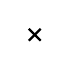
\begin{tikzpicture}
\draw[thick] (0,0) -- (1ex,1ex);
\draw[thick] (1ex,0) -- (0,1ex);
\end{tikzpicture} - Non-orthogonal 
\end{tabular}
}%
%
\providecommand\matlabtextB{\color[rgb]{0.000,0.000,0.000}\fontsize{9}{9}\itshape\selectfont\strut}%
\psfrag{013}[bc][bc]{\matlabtextB Slowness, $\mu$sec/m}%
\psfrag{014}[tc][tc]{\matlabtextB Frequency, kHz}%
%
%% </text>
%
%% <xtick>
%
\def\matlabfragNegXTick{\mathord{\makebox[0pt][r]{$-$}}}
%
\providecommand\matlabtextC{\color[rgb]{0.000,0.000,0.000}\fontsize{9}{9}\selectfont\strut}%
\psfrag{000}[ct][ct]{\matlabtextC $2$}%
\psfrag{001}[ct][ct]{\matlabtextC $4$}%
\psfrag{002}[ct][ct]{\matlabtextC $6$}%
\psfrag{003}[ct][ct]{\matlabtextC $8$}%
%
%% </xtick>
%
%% <ytick>
%
\psfrag{004}[rc][rc]{\matlabtextC $880$}%
\psfrag{005}[rc][rc]{\matlabtextC $900$}%
\psfrag{006}[rc][rc]{\matlabtextC $920$}%
\psfrag{007}[rc][rc]{\matlabtextC $940$}%
\psfrag{008}[rc][rc]{\matlabtextC $960$}%
\psfrag{009}[rc][rc]{\matlabtextC $980$}%
\psfrag{010}[rc][rc]{\matlabtextC $1000$}%
\psfrag{011}[rc][rc]{\matlabtextC $1020$}%
\psfrag{012}[rc][rc]{\matlabtextC $1040$}%
%
%% </ytick>